\documentclass[twoside,11pt]{article}

% Any additional packages needed should be included after jmlr2e.
% Note that jmlr2e.sty includes epsfig, amssymb, natbib and graphicx,
% and defines many common macros, such as 'proof' and 'example'.
%
% It also sets the bibliographystyle to plainnat; for more information on
% natbib citation styles, see the natbib documentation, a copy of which
% is archived at http://www.jmlr.org/format/natbib.pdf

\usepackage{jmlr2e}
\usepackage{multirow}


% Definitions of handy macros can go here

\newcommand{\dataset}{{\cal D}}
\newcommand{\fracpartial}[2]{\frac{\partial #1}{\partial  #2}}

% Heading arguments are {volume}{year}{pages}{submitted}{published}{author-full-names}

% Short headings should be running head and authors last names
%\ShortHeadings{Deep learning from limited data}{Rokem, PhD, Wu, PhD, and Lee, MSc, MD}
\ShortHeadings{Deep learning from limited data}
\firstpageno{1}

\begin{document}

\title{Deep learning from limited amounts of data: a sub-sampling study of classification from optical coherence tomography images}

% \author{\name Ariel Rokem \email arokem@uw.edu \\
%        \addr eScience Institute\\
%        The University of Washington\\
%        Seattle, WA, USA
%        \AND
%        \name Yue Wu  \email wu5@post.harvard.edu \\
%        \addr Department of Ophthalmology\\
%        The University of Washington\\
%        Seattle, WA, USA
%        \AND
%       \name Aaron Lee \email leeay@uw.edu\\
%       \addr Department of Ophthalmology\\
%       The University of Washington\\
%       Seattle, WA, USA}


\author{\name FirstName LastName \email XXX@YYY.ZZZ}
\maketitle

\begin{abstract}

Deep learning has tremendous potential utility in the
classification of biomedical images. For example, images acquired with retinal
optical coherence tomography (OCT) can be used to classify patients
with age-related macular degeneration (AMD), and distinguish them from healthy
control patients. Previous research suggests that large amounts of data are
required in order to train deep learning (DL) algorithms, because of
the large number of parameters that need to be fit. To study the data
requirements of biomedical DL, we applied a subsampling procedure to 
classification of AMD patients from OCT data. We found that performance 
decreases approximately constantly with each halving of the data. These 
results suggest that deep learning algorithms can be trained on
relatively moderate amounts of data, provided that images are homogenous, and 
the effective number of parameters is sufficiently small. Furthermore, we 
demonstrate that in this application, performance evaluation with a separate test set 
that is not used in any part of the training does not differ substantially from 
performance evaluation with a validation data-set that was also used to 
determine the optimal stopping point for training.

\end{abstract}

\section{Introduction}\label{sec:intro}

Deep learning (DL) algorithms \citep{LeCun2015-js} have been tremendously
successful at solving a variety of different computational tasks. Although these
algorithms were originally developed to perform computer vision tasks that
require the identification and classification of natural objects in images
\citep{Krizhevsky2012-az}, they have been more recently successfully applied to
tasks as varied as automated captioning and description of images and
videos\citep{Karpathy2014-nx, Donahue2014-uq}, automated transcription of spoken
language \citep{Hannun2014-uj}, automated translation \citep{Wu2016-kx}, and in
playing games such as Go \citep{Silver2016-uv} and Poker \citep{Hsu2017-cr},
beating even highly seasoned players in these games.

A key to the success of these algorithms in image processing is that they do not
require feature engineering of their front-end filters. Instead, these filters
are empirically learned from the data through a process of training. For
example, a network is trained to identify natural objects by exposing it to
labeled exemplars of images containing the classes to be discriminated. The
weights that define the front-end filters, and their pooling in higher levels
are automatically adjusted through gradient descent. Progress in the
implementation of the computation of the gradients required for this process on
graphical processing units (GPUs) has been instrumental in enabling use of these
techniques on large and complex data-sets. No less important have been the
discovery of network architectures \citep{Canziani2016-ps}, non-linearities
\citep{Glorot2011-hk}, regularization procedures \citep{Hinton2012-fm} and
initialization procedures \citep{Glorot2010-is} that accelerate and improve
learning. Taken together, these factors have ushered in an era where training of
large DL networks has become practical, and there is wide-spread interest in
applying these algorithms to a variety of different tasks.

\subsection{Deep Learning in medical imaging}

Because DL algorithms were originally developed to perform difficult image
processing and classification tasks, one of the compelling avenues for
application of DL is in the analysis of data from medical imaging technologies,
and the development of computer-assisted diagnostic systems with DL-trained
networks at their core. This type of application is rapidly becoming more
realistic because of the combination of high-quality biomedical imaging
technologies that are becoming common in clinical practice, and the development
of large data-sets for the training of these networks. These large data-sets are
the result of years of accumulation of electronic medical records (EMR),
data-bases that include both image data, as well as expert-generated diagnostic
labels. Several recent studies used data from such data-bases in tandem with DL
networks to demonstrate the potential for highly accurate automated diagnosis of
diseases from images of skin lesions \citep{Esteva2017-ho} and chest x-ray
images \citep{Rajpurkar2017-mv}.

Several previous studies demonstrate that DL algorithms are also capable of
accurate diagnosis of a variety of retinal diseases, based on images acquired
using standard clinical instruments \citep{Gulshan2016-fh}. For example,
optical coherence tomography (OCT) images are taken at a high resolution, and
provide information about the three-dimensional structure of the tissue. These
images are routinely collected during clinical ophthalmological visits, and are
normally used by clinicians to assess the presence of retinal diseases, and
determine the appropriate course of treatment. EMR datasets of OCT image data,
together with these expert-generated labels, have been used to demonstrate the
feasibility of automated diagnosis of a variety of conditions
\citep{Gulshan2016-fh, lee2017deep, Lee2017-vp, Awais2017-qw, Kermany2018-bq}.
For example, in a previous study, a VGG16 DL network architecture designed for
object recognition \citep{Simonyan2014-al}, can distinguish OCT scans from
retinae of patients with age-related macular degeneration (AMD) from healthy
retinae with an accuracy of 88.98\% (ROC AUC of 93.83\%, peak sensitivity 92.64
\%, peak specificity 93.69 \%) \citep{lee2017deep}. Here, we use the same
architecture and similar data, to address the question of data requirements for
successful performance.

\subsection{How many samples do you need?}

Previous applications of DL in medical imaging rely on large data sets, that
are not available for many other technologies, and for diseases that are less
common. A major barrier to the wide-spread application of DL algorithms in
medical imaging is the assumption that these algorithms only work well when
data is extremely abundant, and that supervised learning can only progress using
accurate labels of each image\footnote{``As of 2016, a rough rule of thumb is
that a supervised deep learning algorithm will generally achieve acceptable
performance with around 5,000 labeled examples per category, and will match or
exceed human performance when trained with a dataset containing at least 10
million labeled examples.'' \citep{Goodfellow-et-al-2016}, page 20}. Indeed, in
previous work using DL for AMD classification, the network was trained with a
data-set of $\sim$100,000 images \citep{lee2017deep}. Similarly, other studies
have used data-bases with many thousands of patients and up to millions of
individual images \citep{Kermany2018-bq}.

Here, we use a subsampling procedure to assess the decrease in DL
classification performance as a function of the number of samples. We apply this
procedure to empirically evaluate the performance of the VGG16 architecture in
detecting AMD in retinal OCT. To our knowledge, there is only one previous
study asking how many samples are needed in biomedical image classification
\citep{Cho2015data_size}. The authors of this study trained a DL network to
discriminate between six classes of images (brain, neck, shoulder, etc.) from
MRI images. They found that only a few hundred images are required to reach
near-perfect accuracy in this task using the GoogLeNet network. However, images
of these body parts differ in many respects, and it is not clear that a much
simpler algorithm would not perform just as well in this classification task.
We focused instead on a classification task in which DL algorithms are required
to perform more accurately than traditional image processing methods
\citep{Lemaitre2016-gu}. We introduce a subsampling procedure to test the size
of the sample needed in order to train a DL network on a biomedical image
classification task, and use this procedure in order to assess the number of
samples needed to train network to accurately discriminate between AMD and
healthy retinae from OCT.

\subsection{Cross-validation and the importance of a separate test set}

To avoid over-fitting, and to provide an objective and accurate evaluation of
the performance of a classification algorithm, it is common to separate the data
into several different sets: a \emph{training set} is used to learn the
dependencies between input data and model class labels, and to adjust the
parameters of the model. A \emph{validation set} is sometimes used to assess the
current state of the model during training. This is done by feeding a sample or
samples from the validation set through the algorithm, with a fixed set of
parameters, and evaluating the accuracy of the classification with these
parameter values, but without using the results to adjust the parameters.

Often, an additional data set is set aside as \emph{test set}. This set is used
once the learning has ended, to provide an independent evaluation of the 
accuracy of the learning procedure. While using an independent data set guards 
against over-optimism due to over-fitting, it also might introduce 
variability in the estimate of error, especially with a relatively small size 
of the test set \citep{Efron1983-vu}.

In cross-validation, different parts of the data might serve separately as
training and validation data sets \citep{Stone1974-mo}. For example, in k-fold
cross-validation training is repeated several times, where in each iteration
through the procedure, a portion of $N/k$ samples from the data are designated
as a validation set, and the remaining data is used for training. After $k$
repetitions of this procedure, all the data has been used up as validation data.
This means that a full set of errors on the entire data-set has been computed.
This procedure is sometimes used for comparative evaluation of different models,
and for model selection (by comparing cross-validation errors for two or more
models) \citep{Stone1977-ez}.

While this procedure is comprehensive, and potentially reduces variability of
the estimates, it is also computationally demanding. For this reason, training
of DL algorithms usually uses the strategy of training on a subset of the data
and then using other sub-sets for evaluation and testing.  Furthermore, given
the large amounts of data that are often available for training and evaluation,
the final test step is often omitted in applications of DL. For example, in
their highly influential paper on image classification from the ImageNet
dataset, Krizhevsky et al. \citep{Krizhevsky2012-qc} comment that: ``In the
remainder of this paragraph, we use validation and test error rates
interchangeably because in our experience they do not differ by more than
0.1\%''.

The subsampling scheme introduced here also presents an opportunity to evaluate
whether this statement generalizes well to situations in which data is much less
abundant. Therefore, a second aim of the present paper is to assess the use of a
separate test in cross-validation of a DL network.

\section{Methods}

This study was approved by the Institutional Review Board of
the University
% of Washington (UW)
and adhered to the tenets of the Declaration of Helsinki and the Health
Insurance Portability and Accountability Act.

\subsection{Data extraction}
Macular OCT scans were acquired in the course of clinical care, using a
Heidelberg Spectralis OCT scanner (Heidelberg Engineering, Heidelberg, Germany).
High-resolution images of the retinal cross-section were obtained using a
61-line raster scan. All of the images from the period 2006 to 2016 were
extracted using an automated extraction tool from the instrument imaging
database. The images were linked by patient medical record number and dates to
the clinical data stored in EPIC. Specifically, all clinical diagnoses and the
dates of every clinical encounter, macular laser procedure, and intravitreal
injection were extracted from the EPIC Clarity tables.

\subsubsection{Patient and Image Selection}

A normal patient was defined as having no retinal International Classification
of Diseases, 9th Revision (ICD-9) diagnosis and better than 20/30 vision in both
eyes during the entirety of their recorded clinical history at the University. An AMD
patient was defined as having an ICD-9 diagnosis of AMD (codes 362.50, 362.51,f
and 362.52) by a retina specialist, at least 1 intravitreal injection in either
eye, and worse than 20/30 vision in the better-seeing eye. Patients with other
macular pathology by ICD-9 code were excluded. These parameters were chosen
\emph{a priori} to ensure that macular pathology was most likely present in both
eyes in the AMD patients and absent in both eyes in the normal patients.
Consecutive images of patients meeting these criteria were included, and no
images were excluded due to image quality. Labels from the EMR were then linked
to the OCT macular images, and the data were stripped of all protected health
identifiers.

As most of the macular pathology is concentrated in the foveal region, the
decision was made \emph{a priori} to select the central 11 images from each
macular OCT set, and each image was then treated independently, and labeled as
either normal or AMD. The images were histogram equalized and the resolution
down-sampled to 192 by 124 pixels to accommodate RAM limitations.

\subsection{Deep Learning Classification Model}

A modified version of the VGG16 convolutional neural network
\cite{Simonyan2014-al} was implemented using Caffe \cite{jia2014caffe}. This
network was originally designed to classify categories in natural images and was
adapted here to classify healthy and AMD retinae. Weights were initialized using
the Xavier algorithm \cite{Glorot2010-is}. Training was then performed using
multiple iterations, each with a batch size of 100 images. ADAM optimization
\cite{Kingma2014-jl} was used with a starting learning rate of $2 \times
10^{-7}$ and the momentum parameters set to 0.9 and 0.99. The loss of the model
was recorded at each training iteration, and cross-validation with a separate
validation set was conducted every 250 iterations. The training was stopped when
the loss of the model decreased and the accuracy of the validation set
also decreased (indicating that the model was in the over-fitting regime).

\subsection{Sub-sampling experiments}

At the outset of the experiments, a random subset of 10\% of the images were
segregated at the patient level into a separate \emph{test set} of images. These
would be used to test the performance of the DL network at the end of training.
The remaining 90\% of the images were then segregated into 11 replicates of
random subsets of 4\%, 8\%, 16\%, 32\%, 64\%, and 100\% of the available images.
Within each subset, the images were again subdivided into 75\% for training and
25\% for validation. Care was taken to ensure that the validation set and the
training set contained images from a mutually exclusive group of patients (ie,
no single patient contributed images to both the training and validation sets).
The order of images of the training set was then randomized in each replication
condition.

Each replication condition was then trained for a total of 75,000 iterations
and the maximal validation accuracy was recorded. The weights at the time of
the maximal validation accuracy was used to assess the performance of the
network against the held-out test set.

\section{Results}

\subsection{Data and subsampling}

More than 2.6 million optical coherence tomography (OCT) images were extracted
from the imaging database and linked to clinical data from the electronical
medical records (EMR). A total of 48,312 normal OCT scans and 52,690 AMD scans
met the inclusion criteria for use in the training set. At the outset, a test
set was set aside comprising of 9,493 images, to be used only for evaluation of
the training procedure once it is done.

To test the effect of sample size on accuracy of classification with a DL
network, random subsets of 4\%, 8\%, 16\%, 32\%, 64\%, and 100\% were created
from the full dataset, and training was conducted using these different subset
sizes. The breakdown in the number of images in each subset is described in
Table \ref{table_counts}.

\begin{table}[!t]
%% increase table row spacing, adjust to taste
\renewcommand{\arraystretch}{1.1}
% if using array.sty, it might be a good idea to tweak the value of
% \extrarowheight as needed to properly center the text within the cells
\caption{Average image counts for each subset condition}
\label{table_counts}
\centering
%% Some packages, such as MDW tools, offer better commands for making tables
%% than the plain LaTeX2e tabular which is used here.
\begin{tabular}{ccccc}
\hline
\multirow{2}{*}{Subset Percentage} & \multicolumn{2}{c}{Training} & \multicolumn{2}{c}{Validation}  \\
	 & Normal & AMD & Normal & AMD \\
\hline
4\%   & 1,355 & 1,338 & 398 & 374 \\
8\%   & 2,637 & 2,503 & 837 & 815 \\
16\%   & 5,983 & 5,457 & 1,575 & 1,659 \\
32\%   & 10,376 & 10,256 & 3,609 & 3,565 \\
64\%   & 22,692 & 20,574 & 7,247 & 7,059 \\
100\%   & 36,515 & 32,204 & 12,028 & 10,762 \\
\hline
\end{tabular}
\end{table}

\subsection{Learning with different size subsamples}

To assess the robustness of the results to the random selection of specific
images, random subsamples of each one of these proportions were drawn from the
full data-set 11 times. Training of the DL network in each repetition was
allowed to progress for 75,000 iterations. Learning curves, recording validation
accuracy during training are shown in Figure \ref{fig_learning_curves}.

\begin{figure}[!t]
\centering
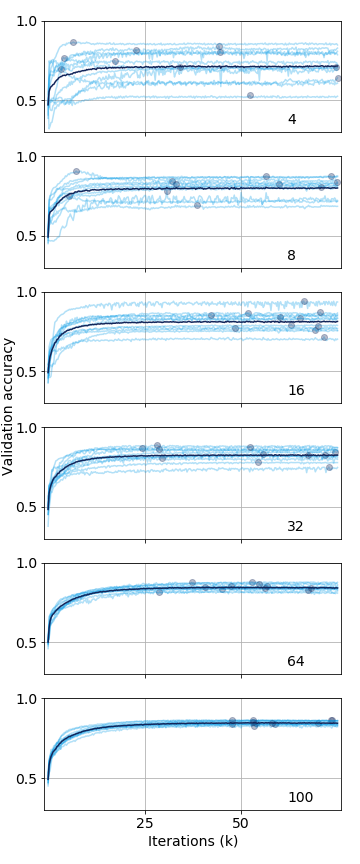
\includegraphics[width=3in]{./figures/learning}

\caption{Learning curves for each subset size (percent). In each sub-plot,
validation accuracy is plotted against number of training iterations. Each of
the repetitions is plotted in light blue, and the average across repetitions is
plotted in dark blue. Maximal validation accuracy in each course of training is
plotted as a light blue point.}

\label{fig_learning_curves}
\end{figure}

\subsection{Test accuracy as a function of subsample size}

For each training run, the weights from the training history with the maximal
validation accuracy were stored. The model was then assessed with these weights
against the held out test set, yielding 11 test accuracy estimates for each
proportion, as seen in Figure \ref{fig_test}. As expected, test accuracy
increased with sample size, reaching its maximal value at subsamples of 100 \%
($\sim$86 \% accuracy).

Though accuracy is far from chance even with only 4 \% of the data ($\sim$73\%
correct) it does increase precipitously between 4\% and 64\% of the data.
However, it reaches close-to-maximal accuracy already at a proportion 16 - 32\%
of the total data-set. To quantify the amount of data needed to reach 95\% of
the maximal accuracy, we fit a two-parameter function, $f(x) = a \cdot log_2(x) + b$,
to the accuracy values across repetitions and sub-sample proportions (orange 
line in figure \ref{fig_test}). Inverting this function, we find that 95\% of 
the maximal accuracy (approximately 82\% accuracy) can already be achieved with 
$\sim30\%$ of the data (dashed lines in \ref{fig_test}).

\begin{figure}[!t]
\centering
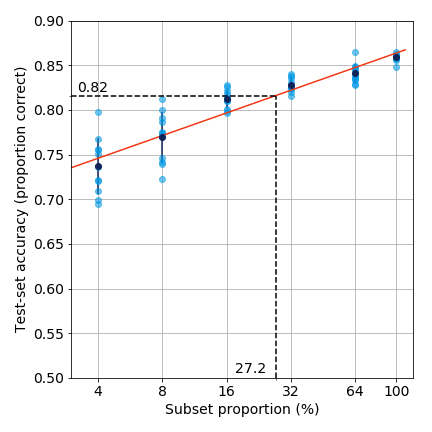
\includegraphics[width=3.5in]{./figures/test}

\caption{Accuracy on held out test set. Weights from the highest validation
accuracy during training were used to test accuracy on a held out test set. Dark
blue points are the means across 11 repetitions, with dark blue standard
deviation error bars. Orange line: a model was fit to all of the sub-samples and 
repetitions. According to this model, 95\% of maximal accuracy
($\sim$82 \% accuracy) can be achieved with 27.2\% of the data (gray lines).}

\label{fig_test}
\end{figure}

\subsection{What explains variability between repetitions?}

Variability of test accuracy also diminished substantially with subsample size.
Differences in variability in the comparisons across different proportions.
These differences in variability could reflect two different factors: the first
is the subsample size, and the other is the degree of overlap between different
subsamples. For example, for 100 \% subsamples, variability reflects only the
random initial conditions of the network, because all subsamples of 100 \% are
identical.  Similarly, the overlap between different subsets in higher
proportions is likely to be larger than in smaller proportions. To evaluate the
effect of this overlap, we conducted a separate experiment in which a single
subset from 4\% group was used, and training was repeated 11 times using the
same set of images, to control for this effect. The learning curves from this
protocol are are shown in Figure \ref{fig_fourpercent}B, together with the
learning curves from random subsamples (Figure \ref{fig_fourpercent}B). The
learning curves have similar variance as when random subsets are used and the
maximal validation accuracy (Figure \ref{fig_fourpercent} C) does not differ
between these protocols. This indicates that variability in test-set accuracy
mostly relates to the size of the subsample, rather than to the amount of
overlap between different subsets.

\begin{figure}[!t]
\centering
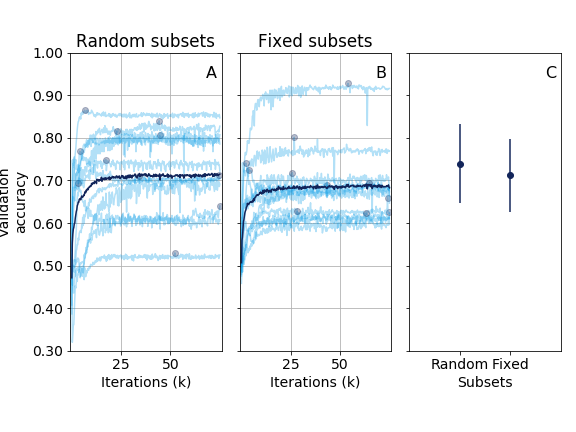
\includegraphics[width=3.5in]{./figures/fourpercent}

\caption{Learning curves of 4\% subset. {\bf A}: Random 4\% subsets of the whole
dataset chosen in each course of learning. {\bf B}: Replications of the same 4\%
susample were repeated in each course of training. {\bf C}: The average maximal
validation accuracies (across the 11 courses of training) are plotted for random
(left) and fixed (subsets) of 4\% each, with standard deviation error bars}

\label{fig_fourpercent}
\end{figure}

\subsection{The importance of a separate test set}

To assess the importance of the separate test set, we computed the difference
between the maximum validation accuracy and test set accuracy (Figure
\ref{fig_diff}). We find that though variability in this difference decreases
with larger sample size, there is no indication that this difference is larger
for smaller sample sizes. In addition, there seems to be no overall bias
indicating that the accuracy is systematically higher for the validation set,
relative to the test set. This indicates that in the training protocol that we
used, there was probably only minimal overfitting, or none at all.

\begin{figure}[!t]
\centering
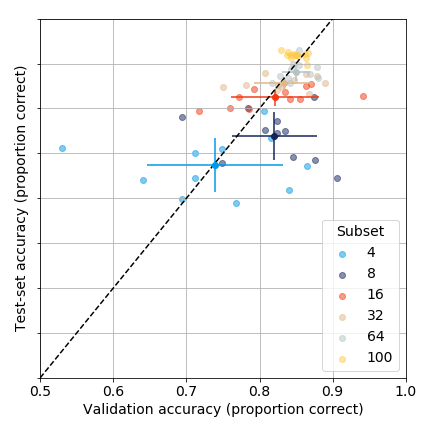
\includegraphics[width=3.5in]{./figures/diff}

\caption{Difference between validation and test accuracy. Each light colored
point represents a single course of training. The abscissa represents the
maximal validation accuracy achieved during this course of training, while the
ordinate represents the accuracy of the network in performing the classification
on a separate test set, using the same weights that resulted in maximal
validation accuracy. Solid colored points each represent the mean across 11
courses of training for each size subset, with standard deviation error bars. 
Dashed line indicates equality.}

\label{fig_diff}
\end{figure}

\section{Discussion and related work}

The application of DL in biomedical imaging is a promising avenue in current
research. Future developments in this field may lead to accurate
computer-assisted diagnosis systems with DL networks at their core.  
A major current impediment to these developments is the assumption that DL 
requires very large data-sets that are not available for many types of nascent 
imaging technologies, or in the case of diseases that are relatively uncommon.

In the present work, we investigated the feasibility of DL with relatively small
sample sizes. We focused on a prototype of computer-assisted diagnosis system
that can accurately discriminate optical coherence tomography (OCT) images from
retinae of patients with age-related macular degeneration AMD, relative to OCT
images from the retinae of healthy controls.

\subsection{How many images do we need to discriminate AMD from healthy retina?}

We found that training a DL network to perform at a high level of accuracy does
not require millions of images. Instead, close-to-maximal performance is
achieved with as few as approximately 20,000 images. Furthermore, the moderate
increase in accuracy from 64\% to 100\% of the data suggests that further
increase in data size would not result in much higher accuracy. This suggests
that $\sim$87\% accuracy is as high as possible with these data and this DL
algorithm. This limit on performance may be related to data quality; the partial
accuracy of the labels in the EMR: these data are heterogeneous and ultimately
depends on clinical decisions made by human observers, as well as the limited
signal-to-noise ratio of the images in capturing the image features that are
diagnostic. However, we do expect further performance improvements to come from
more elaborate algorithms that incorporate additional information, or make
better use of the information in the images, rather than only from more or
better data.

The relatively small number  of images required to train a DL network on this
classification task is surprising given the VGG16 network has as many as 138M
parameters \citep{Canziani2016-ps}. Indeed, previous literature using similar
networks (e.g. \citep{Krizhevsky2012-az, Simonyan2014-al}) used many millions of
training samples to reach high accuracy. The discrepancy between our findings
and the previous literature may stem from the differences between the use-case
we present here, and the common use-case for DL in previous literature. The
assumption that many items from each class are required and that many millions
of separate images are needed to train DL algorithms stems from the object
classification literature mentioned in the introduction, but object
classification in natural images addresses several challenges that are not
typical  in the classification of medical images, and particularly clinical
images from OCT. Primary to these challenges is the variance in pose and
orientation of natural objects within photographic images, which leads to large
variance in the appearance of these objects. To capture all the variations of a
category (e.g., 'dog'), a DL network would have to be exposed to many thousands
of exemplars of this category, generalizing not over all the angles from which
this category could be captured, but also all the sub-categories of this
category (e.g., 'malamut' or 'poodle'). This variance in input is much more
limited in biomedical images, such as OCT. In OCT images, the retina is always
oriented in exactly the same direction, with the macula (the center of the
retina) usually located in roughly the same part of the image. This reduces the
complexity of training substantially, and we hypothesized that it might affect
the data requirements for learning on data such as these.

Nevertheless, given the two-alternative classification task performed here, this
finding is roughly consistent with the rule of thumb described by
\citep{Goodfellow-et-al-2016}(``... 5,000 labeled exemplars per category...'').
The subsampling method introduced here provides a protocol for researchers that
are interested in asking whether they have enough data to apply DL to their
biomedical image data.

Note that because there are 11 images used in each OCT volume, the $\sim$20,000
images represent approximately 1800 volumes of data, or 900 patients per group.
This number of patients is well within range for many traditional random
controlled trials and other clinical studies. This suggests that \emph{de novo}
training of DL networks could be integrated into many studies that are testing
new imaging technologies, or that are studying less common disorders.

\subsection{Other strategies}

There are currently two major alternative strategies to use for cases where data
is limited. Data augmentation synthetically increases the sample size by
performing transformations on the data \citep{Ciresan2011-ko}. This works well
as long as the transformations performed to do not destroy the information
necessary for classification, but introduce variability against which the DL
network should develop tolerance. For clinical imaging data, examples of such
transformations might be rigid translations and rotations of the image features.

The other strategy one might use when faced with limited data is transfer
learning. This strategy is based on the observation that DL algorithms trained
for different image processing tasks often learn very similar first-stage
filters \citep{Bengio2012-nh}. Therefore, in this approach learning begins with
one (larger) data set. This dataset may share only some limited similarity to
the datasets that are ultimately of interest, but this phase of learning allows
the network to converge on good enough front-end filters. Once learning in this
phase has converged, this network is then retrained on the dataset of interest.
This approach is quite promising, and has already been demonstrated to work
well in training a neural network in classification of images from OCT
\citep{Kermany2018-bq}

Both of these approaches are powerful complements to datasets that are not large
enough, but even before employing these strategies, practitioners might want to
assess whether the amount of data that they already have might be sufficient to
accurately learn the classification task at hand.

\subsection{Do we need a separate test set?}

Variance between different courses of training increased substantially with
reduced sample sizes. This variance is not due to sampling of different
individual items --- both average accuracy and variance in accuracy between
repetitions do not change substantially when the same items are repeatedly used
in different subsamples.

Given the limit on test-set accuracy, one might expect that cross-validation on
a separate test-set would be crucial, and that results in the test-set might
differ substantially from the best performance on a validation set
\citep{Zhang_2017}. Nevertheless, we found no systematic difference in
accuracy assessment on a separate test set relative to assessment of accuracy on
a validation set that is repeatedly used during training. This finding is
consistent with previous anecdotal evidence that has been mentioned in the
literature \citep{Krizhevsky2012-qc}.

An important limitation of this conclusion is that in the present study, 
the test set comes from the same pool of images and labels as the training 
and validation sets. In some cases, an independent test set can be acquired 
with a higher (``gold-standard'') level of accuracy. In these cases, it might
still be important to eventually evaluate the performance of the algorithm 
on a separate test set. 

Both of these findings may arise from the large number of parameters that are
fit through the DL algorithm. The learning procedure may thus converge to
different solutions based on initial conditions. When data is small, this may
result in divergent solutions, that depend on the randomly generated initial
conditions of the network. For larger networks, this implies that overfitting is
not induced through repeated use of a validation data-set in accuracy
assessments. However, further research would be needed to assess the limits of
this conclusion and to merit its broad application.


% ACKNOWLEDGEMENTS ONLY GO IN THE CAMERA-READY, NOT THE SUBMISSION
% \acks{We would like to acknowledge NVIDIA Corporation for their generous donation of hardware in support of this research. A. Lee and Y. Wu were supported by an unrestricted grant by the Research to Prevent Blindness to the University of Washington. A. Rokem was supported through a grant from the Gordon & Betty Moore Foundation and the Alfred P. Sloan Foundation to the University of Washington eScience Institute Data Science Environment.}

\bibliography{paper}

\end{document}
